\documentclass[nocover]{pset}
\usepackage{tikz-cd}
\pagestyle{fancy}
\fancyhf{}
\lhead{Forest Kobayashi}
\chead{Basic Category Theory}
\rhead{Math 196 -- Fall, 2018}
\rfoot{\thepage\ of \pageref{LastPage}}
\setlength{\headheight}{15.2pt}
\setlength{\headsep}{10pt}
\lfoot{Thursday, September 20th 2018}

\begin{document}

\begin{center}
  {\scshape \huge Duality in Category Theory}

  {\scshape Lecture 2}
\end{center}
\vspace{-.1cm}
\hrulefill
\begin{adjustwidth}{1em}{1em}
  \section{Introduction}
  First, we'll talk about about some of the hom-set stuff we didn't
  really get much time to touch on last time.
  \subsection{Hom-Sets}
  As as we will see, \emph{hom-sets} play a big role in understanding
  functors. For example, calling a functor \emph{full} is equivalent
  to it being \emph{surjective} on a particular hom-set, and similar
  with faithful functors and injectivity.
  \begin{definition}[Hom-set]
    Let $\mb{C}$ be a category, and $a,b \in \ob(\mb{C})$. Then define
    the \emph{hom-set} of $(a,b)$ by
    \[
      \homm_{\mb{C}}(a,b) = \set{f \mid f \in \homm(\mb{C}),\ f : a
        \to b}.
    \]
  \end{definition}
  This suggests the following (equivalent) formulation of the category
  theory axioms:
  \begin{leftbar}
    {\large \bfseries Category Axioms (hom-set version)}
    \begin{enumerate}[label=(\roman*)]
      \item A small \emph{category} is a set of objects $a,b,c,\ldots$
        together with
      \item A function that assigns to each ordered pair $\ip{a,b}$ a
        set $\homm_{\mb{C}}(a,b)$, and
      \item A function \emph{composition} for each ordered triple
        $\ip{a,b,c}$ with
        \[
          \circ : \homm_{\mb{C}}(b,c) \times \homm_{\mb C}(a,b) \to
          \homm_{\mb C}(a,c)
        \]
      \item For each $b \in \ob(\mb C)$, $\homm_{\mb C}(b,b)$ contains
        at least one element $1_b$ satisfying the ``unit'' axioms
        (see: right / left composition by unit)
      \item Hom-sets are pairwise disjoint. This assures $\dom, \cod$
        are well-defined for all morphisms.
    \end{enumerate}
  \end{leftbar}
  In this context, we can define a functor in terms of hom-sets:
  \begin{definition}[Functor (redux)]
    Let $\mc{T} : \mb{C} \to \mb{B}$ be defined with the usual object
    functor $\mc{T}_o$, together with a collection of functions
    \[
      \mc{T}^{a,b} : \homm_{\mb C}(a,b) \to \homm_{\mb B}(\mc{T}_o(a),
      \mc{T}_o(b))
    \]
    then $\mc{T}$ is \emph{full} when every such $\mc{T}^{a,b}$ is
    surjective, and \emph{faithful} when injective.
  \end{definition}
  On to duality.
  \section{Duality}
  \subsection{Motivation}
  Recall that last time, we defined functors between categories with
  \[
    \mc{T} : \mb{C} \to \mb{B}
  \]
  if
  \[
    \mc{T} =
    \begin{cases}
      \mc{T}_o : \ob(\mb{C}) \to \ob(\mb{B}) &  \\
      \mc{T}_a : \homm(\mb{C}) \to \homm(\mb{B}) &
    \end{cases}
  \]
  such that for all $c \in \ob(\mb{C})$, $\mc{T}(\id_c) =
  \id_{\mc{T}_o(c)}$, and for all $f,g \in \homm(\mb{C})$, $\mc{T}_a
  (g \circ f) = \mc{T}_a(g) \circ \mc{T}_a(f)$. However, as it turns
  out, this is a bit of a restrictive framework --- we could imagine
  plenty of scenarios in which we might want to study something that
  \emph{almost} looks like a functor, except that
  \[
    \mc{T}_a(g \circ f) = \mc{T}_a(f) \circ \mc{T}_a(g).
  \]
  such an object is called a \emph{contravariant} functor, and we will
  examine them in more depth below. But first, note the fundamental
  similarity between the statements above --- if we had objects
  $a,b,c$ with morphisms $f,g,h$ such that the following diagram
  commutes,
  \begin{figure}[H]
    \centering
    \tikzset{node distance=2cm, auto}
    \begin{tikzpicture}
      \node (a) {$a$};
      \node (b) [below of=a] {$b$};
      \node (c) [right of=b] {$c$};
      \draw[-latex] (a) to node {$h = g \circ f$} (c);
      \draw[-latex] (a) to node [swap] {$f$} (b);
      \draw[-latex] (b) to node [swap] {$g$} (c);
    \end{tikzpicture}
    \caption{Example diagram}
  \end{figure}
  then the contravariant functor would create a diagram similar to
  \begin{figure}[H]
    \centering
    \hspace{1.2cm}
    \tikzset{node distance=2cm, auto}
    \begin{tikzpicture}
      \node (a) {$\mc{T}_o(a)$};
      \node (b) [below of=a] {$\mc{T}_o(b)$};
      \node (c) [right of=b] {$\mc{T}_o(c)$};
      \draw[-latex] (c) to node [swap] {$\mc{T}_a(h) = \mc{T}_a(f) \circ
        \mc{T}_a(g)$} (a);
      \draw[-latex] (b) to node {$\mc{T}_a(f)$} (a);
      \draw[-latex] (c) to node {$\mc{T}_a(g)$} (b);
    \end{tikzpicture}
    \caption{Example diagram}
  \end{figure}
  certainly these two structures should be thought of as ``similar''
  in some sense --- if there's any justice in the world, we might even
  expect that some theorems we prove about functors in general will
  translate into guarantees about these so-called ``contravariant
  functors.'' Indeed, this is the case: but to make it formal, we need
  to introduce the idea of \emph{duality}, which will prove
  surprisingly powerful.
  \subsection{Basic definitions}
  As you should now expect, we'll build up from axioms:
  \begin{definition}[Atomic Statements]
    Let $\mb{C}$ be a category. Then if $a,b \in \ob(\mb{C})$, $f,g
    \in \homm(\mb{C})$, an \emph{atomic statement} is a statement of
    the form:
    \begin{enumerate}
      \item $a = \dom(f)$ or $b = \cod(f)$
      \item $\id_a$ is the identity map on $a$
      \item $g$ can be composed with $f$ to yield $h = g \circ f$.
    \end{enumerate}
    That is, an atomic statement is just a statement about the
    axiomatic properties of categories.
  \end{definition}
  From these, we can build phrases of \emph{statements} using the
  formal grammar defined by propositional logic.
  \begin{definition}[Sentences]
    A \emph{sentence} is a statement (see above) in which we have no
    free variables; that is every variable is ``bound'' or
    ``defined.'' For instance, the statement ``for all $f \in
    \homm(\mc{C})$ there exists $a,b \in \ob(\mc{C})$ with $f : a \to
    b$'' forms a sentence, while ``$f : a \to b$'' is an extreme case
    of one that does not (in the latter, we have no idea what any of
    the variables are actually referring to). In the context of
    category theory, the collection of sentences built out of atomic
    statements are known as \emph{ETAC} (``the elementary theory of an
    abstract category'').
  \end{definition}
  Now, we introduce the concept of \emph{duality}:
  \begin{definition}[Duality]
    Let $\Sigma$ be a statement of ETAC. Then the \emph{dual} of
    $\Sigma$ is intuitively the statement ``in reverse,'' and is
    typically denoted by $\Sigma^*$. This can be formalized as simply
    flipping every ``domain'' statement into a ``codomain'' statement,
    and replacing ``$h = g \circ f$'' with ``$h = f \circ g$.'' Some
    examples of duals are given below:
    \begin{table}[H]
      \centering
      \begin{tabular}{@{}lll@{}}
        \toprule
        Statement $\Sigma$ && Dual Statement $\Sigma^*$ \\ \midrule
        $f : a \to b$ && $f : b \to a$  \\
        $a = \dom(f)$ && $a = \cod(f)$ \\
        $i = \id_a$ && $i = \id_a$ \\
        $h = g \circ f$ && $h = f \circ g$ \\
        $f$ is monic && $f$ is epic \\
        $u$ is a right inverse of $h$ && $u$ is a left inverse of $h$
        \\
        $f$ is invertible && $f$ is invertible \\
        $t$ is a terminal object && $t$ is an initial object\\
        \bottomrule
      \end{tabular}
    \end{table}
  \end{definition}
  Note that $\Sigma^{**} = \Sigma$, and that if we prove some theorem
  about a statement $\Sigma$, the dual statement $\Sigma^*$ can be
  proven as well.
  \subsection{Contravariance and Opposites}
  We might ask ourselves: what happens if we dual \emph{every}
  statement in $\mb{C}$? What would some of the resulting objects'
  properties be? This is the focus of the next section.
  \begin{definition}[Dual Category]
    Let $\mb{C}$ be a category. Then call $\mb C^*$ (also denoted
    $\mb C\op$) the \emph{dual} or \emph{opposite} category iff for
    each statement $\Sigma$ about $\mb C$, $\Sigma^*$ holds about $\mb
    C^*$.
  \end{definition}
  This results in the following properties:
  \begin{leftbar}
    {\large \bfseries Properties of the Dual Category}
    \begin{enumerate}[label=\arabic*)]
      \item $\mb C$ and $\mb C^*$ have the same objects.
      \item We can put each $f \in \homm(\mb C)$ into a one-to-one
        relationship with $f^* \in \homm(\mb C^*)$.
      \item For each $f \in \homm(\mb C)$, $\dom(f) = \cod(f^*)$, and
        $\cod(f) = \dom(f^*)$.
      \item For composable $g,f$, $(g \circ f)^* = f^* \circ g^*$.
      \item If $\Sigma^*$ is true in $\mb C$, then $\Sigma$ is true in
        $\mb C^*$.
    \end{enumerate}
  \end{leftbar}
  Recall our definition of contravariant functors on page 2. The
  important quality that we saw with contravariant functors was that
  they \emph{reverse the order} of morphism composition. One might
  note that this sounds an awful lot like a dual property --- and
  indeed, there is a connection here. We examine this in the theorem
  below.
  \begin{theorem}[Contravariant functors and duality]
    Let $\mb C, \mb B$ be categories, and let $T : \mb C \to \mb B$ be
    a contravariant functor. Then $T$ can be expressed as a covariant
    functor from $\mb C^* \to \mb B$
  \end{theorem}
  \begin{proof}
    Let $a,b,c \in \ob(\mb C)$, and let $f : a \to b$, $g : b \to c$.
    Then if $\mc T : \mb C \to \mb B$ is a contravariant functor, let
    $\ol{\mc T} : \mb C^* \to \mb B$ be defined by
    \[
      \mc T f = \ol{\mc T} f^*
    \]
    for all $f \in \homm(\mb C)$. Then note that
    \begin{align*}
      \mc T(g \circ f)
      &= \ol{\mc T} ((g \circ f)^*) \\
      \mc T(f) \circ \mc T(g)
      &= \ol{\mc T} (f^* \circ g^*) \\
      &= \ol{T}(f^*) \circ \ol{T}(g^*)
    \end{align*}
    thus, $\ol{\mc T}$ is a covariant functor from $\mb C^*$ to $\mb
    B$.
  \end{proof}
  similarly, by the principle of duality, any covariant functor from
  $\mb C \to \mb B$ can be thought of as a contravariant functor from
  $\mb C^* \to \mb B$.

  We look at an interesting example:
  \begin{definition}[Hom-functors]
    Let $\mb C$ be a category with small hom-sets. Then since each
    hom-set is small, for every $a \in \ob(\mb C)$, define the
    \emph{covariant hom-functor}
    \[
      \homm_{\mb C}(a, -): \mb C \to \textbf{Set}
    \]
    such that the object function gives
    \[
      b \mapsto \homm_{\mb C}(a,b)
    \]
    and arrow function
    \[
      \bk{k : b \to b'} \mapsto \bk[Big]{\homm_{\mb C}(a,k) :
        \homm_{\mb C}(a,b) \to \homm_{\mb C}(a, b')}
    \]
    where the RHS of the above is defined by $f \mapsto k \circ f$ for
    each $f : a \to b$. Since the notation above is cumbersome,
    MacLane suggests instead using $k_\star$ (``composition with $k$ on
    the left'', or ``the map induced by $k$'').

    Similarly, we define the \emph{contravariant hom-functor} by, for
    each $b \in \ob{\mb C}$,
    \[
      \homm_{\mb C}(-,b) : \mb C^* \to \textbf{Set}
    \]
    with arrow function
    \[
      \bk{g : a \to a'} \mapsto \bk[Big]{\homm_{\mb C}(g, b) :
        \homm_{\mb C}(a',b) \to \homm_{\mb C}(a, b)}
    \]
    defined by $f \mapsto f \circ g$. Again, omitting $b$, this is
    often written as $g^\star$. In summary,
    \[
      k_\star f = k \circ f \qquad g^\star f = f \circ g
    \]
    and the following diagram commutes.
    \begin{figure}[H]
      \centering
      \tikzset{node distance=3cm, auto}
      \begin{tikzpicture}
        \node (a) {$\homm_{\mb C}(a', b)$};
        \node (b) [right of=a] {$\homm_{\mb C}(a,b)$};
        \node (c) [below of=a] {$\homm_{\mb C}(a',b')$};
        \node (d) [below of=b] {$\homm_{\mb C}(a,b')$};
        \draw[-latex] (a) to node [swap] {$k^\star$} (c);
        \draw[-latex] (a) to node {$g_\star$} (b);
        \draw[-latex] (b) to node {$k_\star$} (d);
        \draw[-latex] (c) to node {$g^\star$} (d);
      \end{tikzpicture}
    \end{figure}
  \end{definition}

  \subsection{Products of Categories}
  We define the category analog of the cartesian product:
  \begin{definition}[Product of Categories]
    Let $\mb B, \mb C$ be categories. We construct the \emph{product}
    of $\mb B$ and $\mb C$ as follows:
    \[
      \ob(\mb B \times \mb C) = \ob(\mb B) \times \ob(\mb C)
    \]
    and
    \[
      \homm\pn{\mb B \times \mb C} = \homm\pn{\mb B} \times
      \homm\pn{\mb C}.
    \]
    composition is defined in the obvious manner. For all pairs of
    objects $\ip{b.c}$, $\ip{b', c'}$, $\ip{b'', c''}$, and pairs of
    arrows $\ip{f : b \to b',g : c \to c'}$, $\ip{f' : b' \to b'', g'
      : c' \to c''}$, then if
    \[
      \ip{b,c} \xrightarrow{\ip{f,g}} \ip{b',c'}
      \xrightarrow{\ip{f',g'}} \ip{b'', c''}
    \]
    then we write
    \[
      \ip{f',g'} \circ \ip{f,g} = \ip{f' \circ f, g' \circ g}
    \]
  \end{definition}
  We can define \emph{projection} functors in the obvious manner as
  well:
  \begin{definition}
    Consider functors $P,Q$ with
    \[
      P : \mb B \times \mb C \to \mb B \qquad Q : \mb B \times \mb C
      \to \mb C
    \]
    such that, for all $\ip{f,g} \in \ob(\mb{B \times C}), \homm(\mb{B
    \times C})$,
    \[
      P\ip{f,g} = f, \qquad Q\ip{f,g} = g.
    \]
  \end{definition}
  Here, we will see the first of many descriptions of a ``universal''
  property.
  \begin{theorem}[Look-ahead]
    Let $\mb D$ be a category, and $\mc R$, $\mc T$ be any two
    functors with $\mc R : D \to B$, $\mc T : \mb D \to \mb C$. Then
    $\exists! \mc F : \mb D \to \mb B \times \mb C$ such that the
    following diagram commutes:
    \begin{figure}[H]
      \centering
      \tikzset{node distance=2.5cm, auto}
      \begin{tikzpicture}
        \node (d) {$\mb D$};
        \node (bc) [below of=d] {$\mb B \times \mb C$};
        \node (b) [left of=bc] {$\mb B$};
        \node (c) [right of=bc] {$\mb C$};
        \draw[-latex] (d) -- (b) node[midway, left, xshift=-.25em] {$\mc R$};
        \draw[-latex] (d) -- (c) node[midway, right, xshift=.25em] {$\mc T$};
        \draw[-latex, dotted] (d) -- (bc) node[midway, right]
        {$\mc F$};
        \draw[-latex] (bc) -- (c) node[midway, above left] {$\mc Q$};
        \draw[-latex] (bc) -- (b) node[midway, above right] {$\mc P$};
      \end{tikzpicture}
      \caption{Uniqueness of inclusion}
    \end{figure}
  \end{theorem}
  \begin{proof} (Sketch) For the diagram to commute, for all $h \in
    \homm(\mb D)$, we must have $\mc F = \ip{\mc R h, \mc T h}$. The
    universality follows pretty trivially.
  \end{proof}
  Similarly to products of categories, we define products of functors:
  \begin{definition}[Functor products]
    Let $\mc U : \mb B \to \mb B'$, $\mc V \to \mb C \to \mb C'$. Then
    we say $\mc U$ and $\mc V$ have a product $\mc U \times \mc V :
    \mb B \times \mb C \to \mb B' \times \mb C'$ if
    \[
      (\mc U \times \mc V)_o(\ip{b,c}) = \ip{\mc U_o a, \mc V_o b} \qquad
      (\mc U \times \mc V)_a(\ip{f,g}) = \ip{\mc U_a f, \mc V_a g}
    \]
    equivalently described by the following commutative diagram:
    \begin{figure}[H]
      \centering
      \begin{tikzpicture}
        \node (b) at (-2.5,1) {$\mb B$};
        \node (bc) at (0,1) {$\mb{B \times C}$};
        \node (c) at (2.5,1) {$\mb C$};
        \node (bp) at (-2.5,-1) {$\mb B'$};
        \node (bcp) at (0,-1) {$\mb{B' \times C'}$};
        \node (cp) at (2.5,-1) {$\mb C'$};
        \draw[-latex] (b) -- (bp) node[midway, left] {$\mc U$};
        \draw[-latex, dotted] (bc) -- (bcp) node[midway, right] {$\mc
          U \times \mc V$};
        \draw[-latex] (c) -- (cp) node[midway, right] {$\mc V$};
        \draw[-latex] (bc) -- (c) node[midway, above] {$\mc Q$};
        \draw[-latex] (bc) -- (b) node[midway, above] {$\mc P$};
        \draw[-latex] (bcp) -- (cp) node[midway, above] {$\mc Q'$};
        \draw[-latex] (bcp) -- (bp) node[midway, above] {$\mc P'$};
      \end{tikzpicture}
      \caption{Functor products}
    \end{figure}
  \end{definition}
  Note that since functors are morphisms on categories, then $\times$
  itself is a functor on small categories:
  \[
    \times : \mb{Cat} \times \mb{Cat} \to \mb{Cat}.
  \]
  In the above section, we've concerned ourself with functors mapping
  from a category to a product category (e.g., $\mc F : \mb D \to
  \mb{B \times C}$). We will now examine the ``dual'' concept, that
  functors from a product category to a category.
  \begin{definition}[Bifunctor]
    Let $\mb B$, $\mb C$, $\mb D$ be categories. Let $\mc S : \mb B
    \times \mb C \to \mb D$. Then $\mc S$ is called a
    \emph{bifunctor}.
  \end{definition}

  \begin{theorem}
    Let $\mb{B}, \mb{C}$, and $\mb{D}$ be categories. For all objects
    $c \in \ob(\mb{C})$ and $b \in \ob(\mb{B})$, let
    \[
      \mc{L}_{c} : \mb{B} \to \mb{D}, \qquad \mc{M}_b : \mb{C} \to
      \mb{D}
    \]
    be functors such that $\mc{M}_b(c) = \mc{L}_c(b)$ for all $b$ and
    $c$. Then there exists a bifunctor $\mc{S} : \mb{B} \times \mb{C}
    \to \mb{D}$ with $S(-, c) = \mc{L}_c$ for all $c$ and $S(b, -) =
    \mc{M}_b$ for all $b$ if and only if for every pair of arrows $f :
    b \to b'$ and $g : c \to c'$ one has
    \begin{equation}
      \mc{M}_{b'}(g) \circ \mc{L}_c(f) = \mc{L}_{c'}(f) \circ
      \mc{M}_b(g) \label{eq:tbd}
    \end{equation}
    These equal arrows \ref{eq:tbd} in $\mb{D}$ are then the value
    $\mc{S}(f,g)$ of the arrow function of $\mc{S}$ at $f$ and $g$.
  \end{theorem}
\end{adjustwidth}


\end{document}
